\documentclass{article}
\usepackage{tikz}
\usetikzlibrary{positioning}

\begin{document}

\begin{center}
    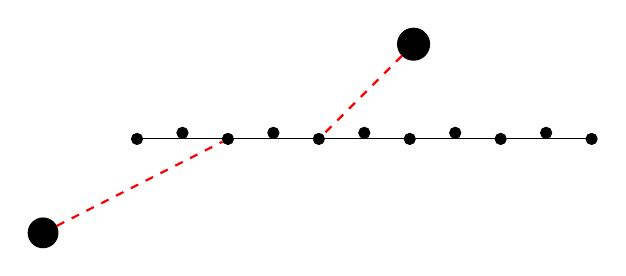
\begin{tikzpicture}[every node/.style={circle, draw, fill=black, inner sep=0pt, minimum size=4pt}]
        \node (0) at (0,0) {};
        \node (1) at (1,0) [right=of 0] {};
        \node (2) at (2,0) [right=of 1] {};
        \node (3) at (3,0) [right=of 2] {};
        \node (4) at (4,0) [right=of 3] {};
        \node (5) at (5,0) [right=of 4] {};

        \path (0) edge node [above] {} (1)
              (1) edge node [above] {} (2)
              (2) edge node [above] {} (3)
              (3) edge node [above] {} (4)
              (4) edge node [above] {} (5);

        \node (u) at (-1,-1) [below left=of 0] {$u_i$};
        \node (v) at (2.5,0.5) [above right=of 2] {$v_j$};

        \draw[red, dashed, thick] (u) -- (1);
        \draw[red, dashed, thick] (v) -- (2);
    \end{tikzpicture}
    \qquad
    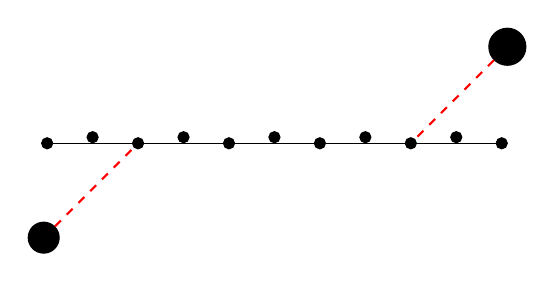
\begin{tikzpicture}[every node/.style={circle, draw, fill=black, inner sep=0pt, minimum size=4pt}]
        \node (0) at (0,0) {};
        \node (1) at (1,0) [right=of 0] {};
        \node (2) at (2,0) [right=of 1] {};
        \node (3) at (3,0) [right=of 2] {};
        \node (4) at (4,0) [right=of 3] {};
        \node (5) at (5,0) [right=of 4] {};

        \path (0) edge node [above] {} (1)
              (1) edge node [above] {} (2)
              (2) edge node [above] {} (3)
              (3) edge node [above] {} (4)
              (4) edge node [above] {} (5);

        \node (w) at (-1,-1) [below left=of 1] {$x_{\ell}$};
        \node (w') at (4.5,0.5) [above right=of 4] {$w_k$};

        \draw[red, dashed, thick] (w) -- (1);
        \draw[red, dashed, thick] (w') -- (4);
    \end{tikzpicture}
\end{center}

The subgraph in \( G'_1 \) formed by adding \((u_i, v_j)\) is isomorphic to the subgraph formed in \( G'_2 \) by adding \((w_k, x_\ell)\). Therefore, in the complements \( G_1 \) and \( G_2 \), removing those edges creates isomorphic graphs.

\end{document}